%%%*******************************************************************************
%  Classe Latex UEFS PPGM, Version 1.0.1 13/09/2021
%
%  Define as normas e estilo das dissertações e teses do PPGM-UEFS
%
%  Author : Gilney Zebende
%  Contribuição : João Paulo Just Peixoto <joao.just@ifba.edu.br,just1982@gmail.com>
%%%-------------------------------------------------------------------------------


%%%-------------------------------------------------------------------------------
%  DOCUMENTAÇÃO COM EXEMPLOS
%%%*******************************************************************************

%%%-------------------------------------------------------------------------------
%%% Thesis default options
%%%-------------------------------------------------------------------------------
%\documentclass[subook]{Classes/PPGM-UEFS}
%\documentclass[sureport]{Classes/PPGM-UEFS}

%%%-------------------------------------------------------------------------------
%%% Thesis custom options
%%%-------------------------------------------------------------------------------

%%% Fancy page headings
%\documentclass[fancyheadings, subook]{Classes/PPGM-UEFS}
%\documentclass[fancyheadings, sureport]{Classes/PPGM-UEFS}

%%% Fancy chapters and sections headings
%\documentclass[fancychapter, subook]{Classes/PPGM-UEFS}
%\documentclass[fancychapter, sureport]{Classes/PPGM-UEFS}

%%% Fancy page , chapters and sections headings
%\documentclass[fancyheadings, fancychapter, subook]{Classes/PPGM-UEFS}
\documentclass[fancyheadings, fancychapter, sureport]{Classes/PPGM-UEFS}


%%%-------------------------------------------------------------------------------
%%% Thesis Commands (ONLY with fancy page headings)
%%%-------------------------------------------------------------------------------

%%%Page header line width
%\footlinewidth{value}

%%%Page footer line width
%\headlinewidth{value}

%%%Page header and footer line width
%\headingslinewidth{value}

%%%Page header and footer lines without text
%\headingslinesonly

%%%The default line width is 0.3pt.
%%%Set the value to 0pt to remove the page header and/or footer line

%%%-------------------------------------------------------------------------------
%%% SUThesis Supported Graphic Formats
%%%-------------------------------------------------------------------------------
% The figures formats supported depend upon the selected output file
% Include your figure without the extention, the SUThesis will automatically
% search the predefined `Figures' directory tree for the right file format.
%
% - The pdfLaTEX (PDF) supports graphics inclusions in PDF, JPG, PNG, and
%   MetaPost (with .mps extention) formats.
%
% - The Latex (DVI) supports graphics inclusions in EPS and PS formats.
%%%-------------------------------------------------------------------------------


%%%-------------------------------------------------------------------------------
%%% Árvore de diretório PPGM-UEFS
%%%-------------------------------------------------------------------------------
%  Diretorio
%       \Classes        (requerido)
%       \Figures        (requerido) --------------------------------->
%       \Figures\PDF    (opcional)
%       \Figures\JPG    (opcional) Figuras nestas pastas
%       \Figures\PNG    (opcional) são buscadas automaticamente
%       \Figures\MPS    (opcional) pela classe PPGM-UEFS.
%       \Figures\EPS    (opcional)
%       \Figures\PS     (opcional) <--------------------------------
%       \Tables         (requerido)
%       \Others         (requerido)
%       \Chapters       (requerido)
%       \Appendices     (opcional)
%       \References     (requerido)
%%%-------------------------------------------------------------------------------

%%%-------------------------------------------------------------------------------
%%% Funções auxiliares (não mude isso)
%%%-------------------------------------------------------------------------------
\newcommand{\nth}[2]{
    \foreach \x [count=\k] in #1 {
        \ifnum\k=#2
            \x
        \fi
    }
}

\makeatletter
\newcommand*\ppgmbancalist{}
\newcommand*\ppgmbancaextlist{}
\newcommand*\ppgmbanca[2]{
    \g@addto@macro\ppgmbancalist{{#1,#2},}
}
\newcommand*\ppgmbancaext[2]{
    \g@addto@macro\ppgmbancaextlist{{#1,#2},}
}
\makeatother

%%%-------------------------------------------------------------------------------
%%% Dados da tese/dissertação
%%%-------------------------------------------------------------------------------
\newif\ifdoutor
\newif\ifcoor

%% Primeiro indique se é uma tese de doutorado ou dissertação de mestrado:
\doutortrue     % Para tese de doutorado
%\doutorfalse   % Para dissertação de mestrado

%% Indique também se tem co-orientador
\coortrue       % Tenho co-orientador
%\coorfalse     % Não tenho co-orientador

%% Preencha as informações abaixo
\newcommand{\ppgmtitulo}       {Título da Dissertação ou Tese}
\newcommand{\ppgmsubtitulo}    {Sub-título da Dissertação ou Tese}
\newcommand{\ppgmautor}        {Nome do(a) autor(a)}
\newcommand{\ppgmorientador}   {Nome do(a) orientador(a)}
\newcommand{\ppgmcoorientador} {Nome do(a) co-orientador(a)}
\newcommand{\ppgmcooruniv}     {UNIVERSIDADE ESTADUAL DE FEIRA DE SANTANA} % Instituição do co-orientador
\newcommand{\ppgmpalavraschave}{palavra-chave1, palavra-chave2, palavra-chave3}
\newcommand{\ppgmkeywords}     {keyword1, keyword2, keyword3}
\newcommand{\ppgmdia}          {Dia}
\newcommand{\ppgmmes}          {Mês}
\newcommand{\ppgmano}          {Ano}
\newcommand{\ppgmcidade}       {Feira de Santana, BA}

%% Indique os membros internos da banca (nome e instituição)
% É possível acrescentar membros copiando o comando
\ppgmbanca{Prof. Dr. Fulano}{\ppgmcooruniv}
\ppgmbanca{Profa. Dra. Beltrana}{\ppgmcooruniv}

%% Indique os membros externos da banca (nome e instituição)
\ppgmbancaext{Prof. Dr. Ciclano}{INSTITUTO FEDERAL DA BAHIA}
\ppgmbancaext{Profa. Dra. Fulana}{UNIVERSIDADE FEDERAL DA BAHIA}


%%%-------------------------------------------------------------------------------
%%% Sumário do PDF
%%%-------------------------------------------------------------------------------
\ifdoutor
    \newcommand{\ppgmsubject}{Tese de Doutorado em Modelagem em Ciências da Terra e do Ambiente}
\else
    \newcommand{\ppgmsubject}{Dissertação de Mestrado em Modelagem em Ciências da Terra e do Ambiente}
\fi

\ifpdf
    \hypersetup{backref,
                colorlinks  = true,
                pdftitle    = \ppgmtitulo,
                pdfauthor   = \ppgmautor,
                pdfsubject  = \ppgmsubject,
                pdfcreator  = PPGM-UEFS,
                pdfproducer = PDFLatex,
                pdfkeywords = \ppgmpalavraschave
    }
\fi

%%%-------------------------------------------------------------------------------
%%% Required packages
%%%-------------------------------------------------------------------------------
% - ifthen
% - setspace
% - amsmath
% - amsfonts
% - amssymb
% - amsthm
% - eucal
% - graphics
% - fancyhdr
%%%-------------------------------------------------------------------------------

%%%-------------------------------------------------------------------------------
%%% Optional packages
%%%-------------------------------------------------------------------------------
%\usepackage[latin1]{inputenc}
\usepackage[utf8]{inputenc}
\usepackage{longtable}
\usepackage{multirow}
\usepackage{lscape}
\usepackage{graphicx}
\usepackage{float,subfigure}
\usepackage{cite}
\usepackage{tikz}
\usepackage{algorithm}
\usepackage{algorithmic}
\usepackage{listings}
\usepackage{lipsum}

%\usepackage{abntex2cite}
\usepackage[alf]{abntex2cite}

\usepackage[left=3cm,top=3cm,right=2cm,bottom=2cm]{geometry}
\usepackage{ifpdf}
% Tables and Figures Caption
\setlength{\LTcapwidth}{\textwidth}

%\newtheorem{theorem}{Teorema}
%\newtheorem{definition}[theorem]{Defini\c{c}\~ao}

\usepackage{hyperref}

% Traduz os títulos dos algoritmos
\makeatletter
\renewcommand{\ALG@name}{Algoritmo}
\renewcommand{\listalgorithmname}{Lista de  \ALG@name s}
\renewcommand{\algorithmicrequire}{\textbf{Entrada:}}
\renewcommand{\algorithmicensure}{\textbf{Saída:}}
\makeatother

%%%-------------------------------------------------------------------------------
%%% Documento raiz da tese/dissertação
%%%-------------------------------------------------------------------------------
\begin{document}
    %%----------------------------------------------------------------------------
    %% Página de título
    %%----------------------------------------------------------------------------
    % Informações da capa. Não é preciso mudar nada aqui.
    \university{UNIVERSIDADE ESTADUAL DE FEIRA DE SANTANA}
    \faculty{Programa de Pós-graduação em Modelagem em Ciências da Terra e do Ambiente}
    
    \ifdoutor
        \course{Doutorado em Modelagem em Ciências da Terra e do Ambiente}
        \typework{Tese de doutorado}
        \thesisdegreetitle{Doutor em Modelagem em Ciências Ambientais}
    \else
        \course{Mestrado em Modelagem em Ciências da Terra e do Ambiente}
        \typework{Dissertação de Mestrado}
        \thesisdegreetitle{Mestre em Mestre em Ciências Ambientais}
    \fi
    
    \thesistitle{\ppgmtitulo}
    \hidevolume
    \thesisvolume{Volume 1 de 1}
    \thesisauthor{\ppgmautor}
    \thesisadvisor{\ppgmorientador}
    \ifcoor
        % Caso não queira exibir o nome do(a) co-orientador(a), habilite a linha abaixo:
        %\hidecoadvisor 
        \thesiscoadvisor{\ppgmcoorientador}
    \fi
    \thesismonthyear{\ppgmmes\space de \ppgmano}
    \maketitlepage

    %%----------------------------------------------------------------------------
    %% Inserir Folha de rosto, Nota de estilo, folha de assinaturas, dedicatória
    %%----------------------------------------------------------------------------
    % Comente qualquer linha que não queira inserir
    %==========================================================
%        Document: PPGM-UEFS
%        File....: FolhaRosto.TEX
%        Author..: Gilney Zebende, João Paulo Just Peixoto
%        Date....: 13 de setembro de 2021
%==========================================================
\begin{folharosto}

\begin{center}
\theauthor
\end{center}
\ \\
\ \\
\ \\
\ \\
\ \\
\begin{spacing}{2}
   \begin{center}
   {\LARGE {\bf \thetitle}}
   \end{center}
\end{spacing}
\ \\
\ \\
\ \\
\begin{flushright}

   \begin{list}{}{
      \setlength{\leftmargin}{4.5cm}
      \setlength{\rightmargin}{0cm}
      \setlength{\labelwidth}{0pt}
      \setlength{\labelsep}{\leftmargin}}

      \item \thetypework apresentada ao \thefaculty, Curso de \thecourse
      da \theuniversity, como requisito parcial para a obtenção do
      título de {\bf \thedegreetitle}.

    \begin{list}{}{
      \setlength{\leftmargin}{0cm}
      \setlength{\rightmargin}{0cm}
      \setlength{\labelwidth}{0pt}
      \setlength{\labelsep}{\leftmargin}}

      \item Área de conhecimento: Estudos Ambientais e Geotecnologias

      \item Orientador: Dr. \theadvisor
      \newline \hspace*{2.1cm}  {\footnotesize {\it \theuniversity}}
      
      \ifcoor
          \item Co-orientador: Dr. \thecoadvisor
          \newline \hspace*{2.1cm}  {\footnotesize \emph{\ppgmcooruniv}}
      \fi
      \end{list}
   \end{list}

\end{flushright}

\vspace*{\fill}

%\begin{spacing}{1.5}
   \begin{center}
   \ppgmcidade \par
   \theuniversity \par
   \ppgmano
   \end{center}
%\end{spacing}

\end{folharosto}

    %==========================================================
%        Document: PPGM-UEFS
%        File....: NotaEstilo.TEX
%        Author..: Gilney Zebende
%        Date....: 24 de abril de 2018
%==========================================================

\begin{notaestilo}
Esta \thetypeworkthree foi elaborada considerando as normas de estilo propostas e aprovadas pelo colegiado do \thefacultytwo e est\~ao dispon\'iveis no formato eletr\^onico (\url{http://ppgm.uefs.br/banco-de-dissertacoes}) ou no formato impresso para consulta. \\


\end{notaestilo}

    %==========================================================
%        Document: PPGM-UEFS
%        File....: FolhaAssinaturas.TEX
%        Author..: Gilney Zebende, João Paulo Just Peixoto
%        Date....: 14 de setembro de 2021
%==========================================================

\begin{folhaassinaturas}

%\thispagestyle{empty}

\def\signature#1#2{\parbox[b]{1in}{\smash{#1}\vskip12pt}
\hfill \parbox[t]{4in}{\shortstack{\vrule width 4in height
0.4pt\\\small#2}}}

\def\InstituicaoMembro#1#2{\parbox[b]{1in}{\smash{#1}\vskip12pt}
\hfill \parbox[t]{4in}{\shortstack{\vrule width 4in \\\small#2}}}

\def\signaturepage{%

    \begin{spacing}{1.5}
        \begin{center}
        {\LARGE \theuniversity} \\
        {\large \thefaculty} \\
        {\large \thecourse} \\
        \end{center}
    \end{spacing}

   \vskip 0.25in plus 0.4in minus 0.1in

    \begin{spacing}{1.0}
        \begin{sloppypar}
        A Banca Examinadora, constitu\'ida pelos professores listados abaixo, leu e recomenda a aprova\c{c}\~ao da
        \thetypeworktwo, intitulada ``\thetitle'',
        apresentada no dia (dia) de (m\^es) de (ano), como requisito
        parcial para a obten\c{c}\~ao do t\'itulo de {\bf \thedegreetitle}.\\
        \end{sloppypar}
    \end{spacing}

    \def\sigskip{\vskip0.15in plus 0.2in minus 0.1in}
    \def\beginskip{\vskip0.3875in plus 0.2in minus 0.1in}

    \beginskip
    \signature{Orientador:}{Prof. Dr. \theadvisor} \\
    \InstituicaoMembro{}{\theuniversity} \\

    \ifcoor
        \sigskip
        \beginskip
        \signature{Co-Orientador:}{Prof. Dr. \thecoadvisor} \\
        \InstituicaoMembro{}{\ppgmcooruniv} \\
    \fi

    \foreach \i in \ppgmbancaextlist {
        \ifx\i\empty{}
        \else
            \sigskip
            \beginskip
            \signature{Membro externo da Banca:}{\nth{\i}{1}} \\
            \InstituicaoMembro{}{\nth{\i}{2}} \\
        \fi
    }
    
    \foreach \i in \ppgmbancalist {
        \ifx\i\empty{}
        \else
            \sigskip
            \beginskip
            \signature{Membro interno da Banca:}{\nth{\i}{1}} \\
            \InstituicaoMembro{}{\nth{\i}{2}} \\
        \fi
    }

    \vfill
    \newpage
    \setcounter{page}{3}
}
%*********************************************************************


\signaturepage


\end{folhaassinaturas}

    %==========================================================
%        Document: PPGM-UEFS
%        File....: Dedicatoria.TEX
%        Author..: Gilney Zebende, João Paulo Just Peixoto
%        Date....: 14 de setembro de 2021
%==========================================================

\begin{dedicatoria}
%\thispagestyle{empty}

\vspace*{\fill}

\begin{flushright}
Dedico este trabalho a...
\end{flushright}
\end{dedicatoria}

    %==========================================================
%        Document: PPGM-UEFS
%        File....: Agradecimentos.TEX
%        Author..: Gilney Zebende
%        Date....: 24 de abril de 2018
%==========================================================
% Neste arquivo de agradecimentos é preciso usar \\ para saltar parágrafos.

\begin{agradecimentos}

\ \\
Ao Prof. Dr. \theadvisor, pela orientação e dedicação ao tema escolhido, e por ter acreditado na pesquisa .\\
\\
Ao Prof. Dr. Fulano de Tal.\\
\\
Ao colega João Paulo, por ter me ensinado a usar o \LaTeX.\\
\\
A UEFS e ao PPGM pelos recursos proporcionados para a elaboração da pesquisa\\
\\

\noindent
\ppgmcidade, Brasil \hfill \theauthor\\
\ppgmdia\space de \ppgmmes\space de \ppgmano
\end{agradecimentos}


    %%----------------------------------------------------------------------------
    %% Resumo/abstract, sumário e siglas
    %%----------------------------------------------------------------------------
    % Comente qualquer linha que não queira inserir
    \begin{romanpagenumbers}
        % Resumo e abstract
        \begin{thesisresumo}

Escreva aqui o seu resumo em português.\\

\textbf{Palavras Chaves:} \ppgmpalavraschave

\end{thesisresumo}

        \begin{thesisabastract}

Write here your abstract in english.\\

\textbf{Keywords:} \ppgmkeywords

\end{thesisabastract}

        
        % Sumários
        \thesiscontents
        
        % Lista de algoritmos (remova se seu texto não possuir algoritmos)
        \listofalgorithms
        
        % Abreviações
        \begin{thesisabbreviations}
\begin{footnotesize}
\begin{longtable}[l]{p{2cm}l}

    %%% Lista de siglas e abreviações
    % Faça conforme o modelo:
    %
    % SIGLA \dotfill & Descrição da sigla \\
    UEFS    \dotfill & Universidade Estadual de Feira de Santana \\
    PPGM    \dotfill & Programa de Pós-Graduação em Modelagem em Ciências da Terra e do Ambiente \\
    CAPES   \dotfill & Coordenação de Aprefeiçoamento de Pessoal de Nível Superior \\
    DCCA    \dotfill & \emph{Detrended Cross-Correlation Analysis} \\
    DFA     \dotfill & \emph{Detrended Fluctuation Analysis} \\
    WWW     \dotfill & \emph{World Wide Web} \\

\end{longtable}
\end{footnotesize}
\end{thesisabbreviations}


        % Volta à numeração de página padrão
    \end{romanpagenumbers}

    %%----------------------------------------------------------------------------
    %% Inclui capítulos da tese/dissertação
    %%----------------------------------------------------------------------------
    \parskip=\baselineskip
    % Comente qualquer linha que não queira inserir
    \chapter{Introdução}
\label{cap:introducao}

Bem-vindo(a) ao modelo de teses e dissertações do PPGM. Neste texto você aprenderá os comandos básicos para escrever sua tese ou dissertação no \LaTeX. O texto em PDF explica a utilização básica e ensina um pouco de \LaTeX, enquanto você pode abrir os arquivos \verb=.tex= para ver como cada coisa é feita. Geralmente o resultado de cada comando será exibido logo abaixo do exemplo do comando.

ATENÇÃO: Ao abrir os arquivos \verb=.tex= você irá se deparar com os comandos \verb=\verb= e os ambientes \verb=verbatim=. Eles são usados para exibir os comandos no texto final em PDF. Ignore-os.

Sempre comece um capítulo com o comando \verb=\chapter{}=, indicando o título do capítulo entre chaves. Para facilitar possíveis citações ao capítulo, use também o comando \verb=\label{}= logo após o título do capítulo, especificando uma chave para essa seção. Veja o exemplo logo no início deste arquivo.

Seções e sub-seções dentro de um capítulo podem ser criadas com os comandos \verb=\section{}= e \verb=\subsection{}= respectivamente. Novamente, sempre crie um \verb=\label{}= nas seções e sub-seções... pode ser que você precise lá na frente. Exemplo:

\begin{verbatim}
    \chapter{Introdução}
    \label{cap:introducao}
    
    Sempre comece um capítulo com o comando...
    
    \section{Como usar essa citação?}
    \label{sec:como_usar_essa_citacao}
    
    Suponha que você queira citar este capítulo...
\end{verbatim}

A seguir iremos entender os comandos mais comuns do \LaTeX\space para este modelo de tese e dissertação do PPGM.

\section{Como usar essa citação?}
\label{sec:como_usar_essa_citacao}

Suponha que você queira citar este capítulo em alguma parte do texto. Basta usar o comando \verb=\ref{}= e informar a chave criada no \verb=\label{}=. Veja o exemplo a seguir e observe o resultado no PDF:

\begin{verbatim}
    ...conforme demonstrado no Capítulo~\ref{cap:introducao}.
\end{verbatim}

...conforme demonstrado no Capítulo~\ref{cap:introducao}.

O til entre a palavra ``Capítulo'' e o comando \verb=\ref{}= serve pra impedir que os dois fiquem em linhas diferentes.

\subsection{O que é uma sub-seção?}
\label{subsec:o_que_e_subsecao}

Este é um exemplo de uma sub-seção. Use quando for necessário.

\subsection{Existe uma regra para nomear os labels?}
\label{subsec:regra_labels}

Não existe uma regra rígida, mas algumas pessoas (como eu) gostam de acrescentar uma sigla indicando o tipo de citação (\verb=cap:= para capítulos, \verb=sec:= para seções, \verb=subsec:= para sub-seções, \verb=tab:= para tabelas e \verb=img:= para imagens).

Esse formato não é obrigatório, mas ajuda na hora de lembrar as chaves e de entender ao que ela se refere quando encontrada no texto.

\section{Listas}
\label{sec:listas}

Usamos listas para enumerar itens no texto. As listas podem ser não ordenadas ou ordenadas.

\subsection{Listas não ordenadas}
\label{sec:listas_nao_ordenadas}

As listas não ordenadas são feitas usando o ambiente \verb=itemize=. Cada item da lista é adicionado com o comando \verb=\item= dentro do ambiente.

É possível criar uma hierarquia de itens (como sub-itens) adicionando outro ambiente \verb=itemize= dentro do já existente. Veja o exemplo abaixo, ele contém três itens, sendo que o segundo contem um sub-item:

\begin{verbatim}
    \begin{itemize}
        \item Este é o primeiro item da lista.
        \item Agora temos o segundo.
        \begin{itemize}
            \item Também podemos ter uma hierarquia de itens.
        \end{itemize}
        \item E podemos ter quantos quisermos.
    \end{itemize}    
\end{verbatim}

\begin{itemize}
    \item Este é o primeiro item da lista.
    
    \item Agora temos o segundo.
    
    \begin{itemize}
        \item Também podemos ter uma hierarquia de itens.
    \end{itemize}
    
    \item E podemos ter quantos quisermos.
\end{itemize}

O próprio \LaTeX\space cuidará de alinhar os itens e seus sub-itens.

\subsection{Listas ordenadas}
\label{sec:listas_ordenadas}

As listas ordenadas são feitas usando o ambiente \verb=enumerate= e segue a mesma lógica das listas não ordenadas, com itens e sub-itens.

\begin{verbatim}
    \begin{enumerate}
        \item Este é o primeiro item da lista.
        \item Agora temos o segundo.
        \begin{enumerate}
            \item Também podemos ter uma hierarquia de itens.
        \end{enumerate}
        \item E podemos ter quantos quisermos.
    \end{enumerate}    
\end{verbatim}

\begin{enumerate}
    \item Este é o primeiro item da lista.
    
    \item Agora temos o segundo.
    
    \begin{enumerate}
        \item Também podemos ter uma hierarquia de itens.
    \end{enumerate}
    
    \item E podemos ter quantos quisermos.
\end{enumerate}

Este foi o mesmo exemplo das listas não ordenadas, porém trocando o \verb=itemize= por \verb=enumerate=.

\section{Figuras}
\label{sec:figuras}

As figuras são inseridas com o ambiente \verb=figure=, acrescentando algumas opções.

Logo após o início do ambiente \verb=figure=, as opções \verb=[htb]= indicam a posição da figura.

\begin{itemize}
    \item \verb=h= para ``aqui'' (here).
    \item \verb=t= para ``top'' (no topo desta ou da próxima página, de acordo com o espaço).
    \item \verb=b= para ``bottom'' (no final desta ou da próxima página, de acordo com o espaço).
\end{itemize}

É possível combinar as opções, por exemplo: \verb=[htb]=, para que o \LaTeX\space tente a melhor posição dentre as três opções.

Dentro do ambiente \verb=figure= usamos alguns comandos:

\begin{itemize}
    \item O comando \verb=\centering= serve para centralizar a imagem.
    \item O comando \verb=\includegraphics[]{}= indica o arquivo com a imagem. Pode ser JPG, PNG, SVG, TIFF, PDF... Recomendo usar imagens em formato vetorial para uma melhor qualidade, como PDF, SVG ou TIFF.
    \item O comando \verb=\caption{}= define a legenda da imagem. Ela será numerada automaticamente.
    \item O comando \verb=\label{}= vai dar uma chave para imagem, de forma que possamos referenciá-la (lembra do início do capítulo?)
\end{itemize}

O exemplo a seguir insere uma figura com essas opções acima:

\begin{verbatim}
    \begin{figure}[h]
    	\centering
    	
\includegraphics{Figures/droopy.jpg}
    	\caption{Primeiro exemplo de figura.}
    	\label{fig:exemplo_1}
    \end{figure}
\end{verbatim}

\begin{figure}[h]
	\centering
	
\includegraphics{Figures/droopy.jpg}
	\caption{Primeiro exemplo de figura.}
	\label{fig:exemplo_1}
\end{figure}

A Figura~\ref{fig:exemplo_1} aparecerá conforme o exemplo acima.

Podemos também alterar o tamanho da figura com a opção \verb=scale= do comando\linebreak \verb=\includegraphics[]{}=, determinando a escala. Dessa forma o \LaTeX\space redimensiona sem perder a proporção. Na Figura~\ref{fig:exemplo_2} a mesma imagem aparece com a metade do tamanho. O código a seguir executa esta tarefa:

\begin{verbatim}
    \begin{figure}[h]
    	\centering
    	
\includegraphics[scale=0.5]{Figures/droopy.jpg}
    	\caption{Primeiro exemplo de figura.}
    	\label{fig:exemplo_1}
    \end{figure}
\end{verbatim}

\begin{figure}[h]
	\centering
	
\includegraphics[scale=0.5]{Figures/droopy.jpg}
	\caption{Figura com a metade do tamanho em escala.}
	\label{fig:exemplo_2}
\end{figure}

Outras formas de ajustes podem ser encontradas no endereço \url{http://latexbr.blogspot.com/2011/07/inserindo-figuras-no-latex.html}.

\section{Tabelas}
\label{sec:tabelas}

Tabelas podem ser chatas de fazer no \LaTeX, pois precisamos especificar toda sua configuração manualmente, até mesmo cada borda.

As tabelas funcionam dentro do ambiente \verb=table= e seguem as opções de posicionamento assim como as figuras. Também usamos o comando \verb=\centering= para centralizar, além dos comandos \verb=\caption{}= e \verb=\label{}=, para dar uma legenda e uma referência, respectivamente. Pelas normas da ABNT, as tabelas devem seguir o padrão do IBGE: o título da tabela deve ficar no topo e a fonte, se for especificada, abaixo, conforme exibido na Tabela~\ref{tab:personagens}.

Dentro do ambiente \verb=table= vem o ambiente \verb=tabular{}=, que irá dizer quantas colunas a tabela terá, as bordas laterais e o alinhamento das células. A quantidade de colunas é definida pelas letras entre as chaves (\verb=l= para alinhado à esquerda, \verb=c= para centralizado e \verb=r= para alinhado à direita). Uma barra | entre as letras indica uma borda vertical na coluna.

Criar tabelas manualmente no \LaTeX\space pode ser complicado, por isso, recomendo usar a ferramenta online no endereço \url{https://www.tablesgenerator.com/}. Lá, você poderá montar a tabela usando uma ferramenta visual e gerar o código \LaTeX\space correspondente. A Tabela~\ref{tab:personagens} foi gerada usando os comandos a seguir:

\begin{verbatim}
    \begin{table}[h]
        \centering
        \caption{Personagens de \emph{The Big Bang Theory} e suas
        áreas de atuação.}
        \label{tab:personagens}
        \begin{tabular}{ll}
            \hline
            \textbf{Personagem} & \textbf{Área de atuação}  \\ \hline
            Sheldon Cooper      & Física Teórica            \\
            Leonard Hofstadter  & Física Experimental       \\
            Howard Wolowitz     & Engenharia Aeroespacial   \\
            Rajesh Koothrappali & Astrofísica de partículas \\ \hline
        \end{tabular}
        \linebreak
        Fonte: \emph{Internet.}
    \end{table}
\end{verbatim}

\begin{table}[h]
    \centering
    \caption{Personagens de \emph{The Big Bang Theory} e suas áreas de atuação.}
    \label{tab:personagens}
    \begin{tabular}{ll}
        \hline
        \textbf{Personagem} & \textbf{Área de atuação}  \\ \hline
        Sheldon Cooper      & Física Teórica            \\
        Leonard Hofstadter  & Física Experimental       \\
        Howard Wolowitz     & Engenharia Aeroespacial   \\
        Rajesh Koothrappali & Astrofísica de partículas \\ \hline
    \end{tabular}
    \linebreak
    Fonte: \emph{Internet.}
\end{table}

\section{Quadros}
\label{sec:quadros}

Os quadros são como as tabelas, porém, possuem todas as linhas de bordas (diferente da tabela, que segue um padrão do IBGE, o quadro é todo fechado).

O funcionamento é o mesmo das tabelas, porém, iremos usar o ambiente \verb=quadro=, conforme abaixo:

\begin{verbatim}
    \begin{quadro}
        \centering
        \caption{Datas das publicações}
        \label{qua:publicacoes}
        \begin{tabular}{|c|c|}
            \hline
            \textbf{Título}                     & \textbf{Ano} \\
            \hline
            Emergências em cidades: uma revisão & 2021 \\
            \hline
            Propostas para mobilidade urbana    & 2022 \\
            \hline
        \end{tabular}
        \linebreak
        Fonte: \emph{Internet}.
    \end{quadro}
\end{verbatim}

\begin{quadro}
    \centering
    \caption{Datas das publicações}
    \label{qua:publicacoes}
    \begin{tabular}{|c|c|}
        \hline
        \textbf{Título}                     & \textbf{Ano} \\
        \hline
        Emergências em cidades: uma revisão & 2021 \\
        \hline
        Propostas para mobilidade urbana    & 2022 \\
        \hline
    \end{tabular}
    \linebreak
    Fonte: \emph{Internet}.
\end{quadro}

Assim como no caso das tabelas, será criada uma lista de quadros no início do documento.

\section{Equações}
\label{sec:equacoes}

Para as equações, usaremos o ambiente \verb=equation=. Basta abrir o ambiente, definir a referência com um \verb=\label{}= e digitar a equação, conforme o exemplo a seguir:

\begin{verbatim}
    \begin{equation}
        \label{eq:funcao_linear}
        f(x) = 2x + 5
    \end{equation}
\end{verbatim}

\begin{equation}
    \label{eq:funcao_linear}
    f(x) = 2x + 5
\end{equation}

É possível fazer equações de qualquer tipo, basta saber os comandos corretos. No endereço \url{https://en.wikibooks.org/wiki/LaTeX/Mathematics} você tem uma lista de vários comandos específicos para equações matemáticas. Veja alguns exemplos em funcionamento a seguir:

\begin{equation}
    \label{eq:gravidade}
    F = G \cdot \frac{m_1 \cdot m_2}{r^2}
\end{equation}

\begin{equation}
    \label{eq:limites}
    \lim\limits_{x \to 0} f\left(\frac{1}{x}\right) = \infty
\end{equation}

\begin{equation}
    \label{eq:somatorio}
    T = \sum_{i=1}^{n} t_i
\end{equation}

Caso queira inserir uma equação dentro do texto, escreva-a entre dois símbolos de cifrão:

\begin{verbatim}
    ...e então, Albert Einstein chegou à famosa equação $E = mc^2$,
    que todos conhecem.
\end{verbatim}

...e então, Albert Einstein chegou à famosa equação $E = mc^2$, que todos conhecem.

\section{Algoritmos}
\label{sec:algoritmos}

Os ambientes \verb=algorithm= e \verb=algorithmic= permitem a escrita de pseudocódigos no documento \LaTeX. Esses ambientes requerem alguns comandos especiais, como descrito em \url{https://en.wikibooks.org/wiki/LaTeX/Algorithms}. Abaixo, um exemplo de um algoritmo de busca:

\begin{verbatim}
    \begin{algorithm}
    \caption{Algoritmo recursivo de busca binária.}
    \begin{algorithmic}
        \REQUIRE $v \gets$ vetor, $n \gets$ tamanho, $x \gets$ elemento
        \ENSURE $p \gets$ posição
        \STATE $p \gets n/2$
        \STATE $y \gets v[p]$
        \IF{$y = x$}
            \RETURN $p$
        \ELSE
            \IF{$x < $y}
                \RETURN $busca(v, n/2, x)$
            \ELSE
                \RETURN $busca(v[n/2], n/2, x)$
            \ENDIF
        \ENDIF
    \end{algorithmic}
    \end{algorithm}
\end{verbatim}

\begin{algorithm}
\caption{Algoritmo recursivo de busca binária.}
\begin{algorithmic}
    \REQUIRE $v \gets$ vetor, $n \gets$ tamanho, $x \gets$ elemento
    \ENSURE $p \gets$ posição
    \STATE $p \gets n/2$
    \STATE $y \gets v[p]$
    \IF{$y = x$}
        \RETURN $p$
    \ELSE
        \IF{$x < $y}
            \RETURN $busca(v, n/2, x)$
        \ELSE
            \RETURN $busca(v[n/2], n/2, x)$
        \ENDIF
    \ENDIF
\end{algorithmic}
\end{algorithm}

Caso queira escrever código em alguma linguagem de programação específica, use o ambiente \verb=lstlisting= dentro do ambiente de algoritmo. O \LaTeX\space irá fazer alguns destaques no texto para facilitar a leitura do código-fonte, conforme o exemplo a seguir:

\begin{verbatim}
    \begin{algorithm}
    \caption{Exemplo em Python.}
    \label{alg:python}
    \begin{lstlisting}[language=Python]
    nome = input("Qual seu nome?")
    print(f"Oi, {nome}!")
    \end{lstlisting}
    \end{algorithm}
\end{verbatim}

\begin{algorithm}
\caption{Exemplo em Python.}
\label{alg:python}
\begin{lstlisting}[language=Python]
nome = input("Qual seu nome?")
print(f"Oi, {nome}!")
\end{lstlisting}
\end{algorithm}

Finalmente, também é possível carregar o código de um arquivo, sem a necessidade de escrever o código por completo no \LaTeX. Neste caso, basta indicar o arquivo com o comando \verb=\lstinputlisting[]{}=, conforme o exemplo abaixo. Detalhe: o arquivo precisa estar na pasta do projeto.

\begin{verbatim}
    \begin{algorithm}
    \caption{Arquivo codigo.py}
    \label{alg:codigo_py}
    \lstinputlisting[language=Python]{codigo.py}
    \end{algorithm}
\end{verbatim}

\section{Referências bibliográficas}
\label{sec:referencias_bibliograficas}

O \LaTeX\space auxilia bastante no uso das referências bibliográficas, portanto, não será mais preciso se preocupar em verificar quais referências foram usadas para listá-las na seção de Referências. Usaremos o BibTeX em conjunto com alguns comandos para fazer esse gerenciamento.

\subsection{BibTeX}
\label{subsec:bibtex}

O BibTeX é uma ferramenta para referências no \LaTeX. Ele também possui uma linguagem própria para especificação dos documentos referenciados. Veja um exemplo a seguir:

\begin{verbatim}
@article{Costa2020,
   author  = {Daniel G. Costa and João Paulo J. Peixoto},
   doi     = {10.1049/iet-smc.2020.0044},
   issn    = {2631-7680},
   issue   = {2},
   journal = {IET Smart Cities},
   title   = {COVID‐19 pandemic: a review of smart cities initiatives to
              face new outbreaks},
   volume  = {2},
   year    = {2020},
}
\end{verbatim}

Cada documento no BibTeX inicia com o seu tipo (neste caso, \verb=@article= para um artigo). Logo em seguida, vem a chave do documento. Essa é a chave que usaremos para citar o artigo no nosso texto. No exemplo acima, a chave é \verb=Costa2020=. Em seguida, nas linhas seguintes, vêm os dados do artigo, como autores, título, ano, etc.

Não se preocupe, não será preciso aprender mais uma linguagem. Você pode (e deve) usar ferramentas para gerenciar suas referências, como o JabRef, Mendeley e outros. Além disso, a maioria dos \emph{sites} já fornecem as referências em BibTeX.

No Google Acadêmico, clique no ícone de aspas abaixo do \emph{abstract} do artigo. Uma nova janela aparecerá, conforme a Figura~\ref{fig:bibtex_google}. Clique em ``BibTeX'' para receber a referência.

\begin{figure}[h]
    \centering
    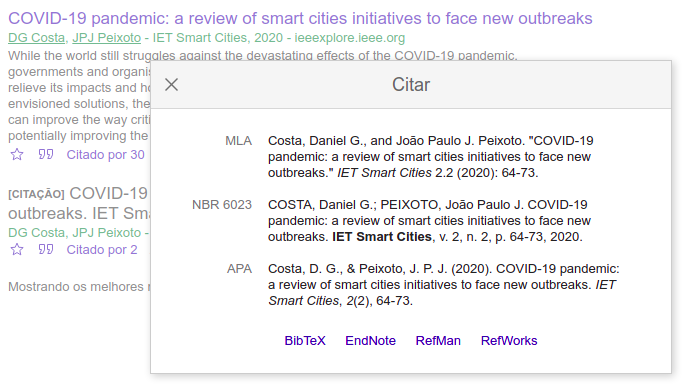
\includegraphics[scale=0.5]{Figures/bibtex_google.png}
    \caption{Opção para citação em BibTeX no Google Acadêmico.}
    \label{fig:bibtex_google}
\end{figure}

No Mendeley Web, selecione os artigos que deseja exportar e clique no botão ``Export'' na barra inferior. Um menu irá abrir com a opção de exportar no formato BibTeX, conforme mostra a Figura~\ref{fig:bibtex_mendeley}.

\begin{figure}[h]
    \centering
    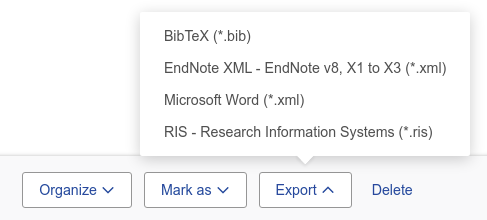
\includegraphics[scale=0.5]{Figures/bibtex_mendeley.png}
    \caption{Menu de exportação no Mendeley com suporte a BibTeX.}
    \label{fig:bibtex_mendeley}
\end{figure}

Se estiver usando o Mendeley Desktop, é preciso habilitar a opção de sincronia BibTeX na janela de opções. Nesta tela você deverá marcar as opções conforme a Figura~\ref{fig:bibtex_mendeley_desktop}. Em ``Path'', selecione a pasta onde quer salvar o arquivo \verb=.bib= e o Mendeley irá salvar automaticamente com o nome \verb=library.bib=.

\begin{figure}[h]
    \centering
    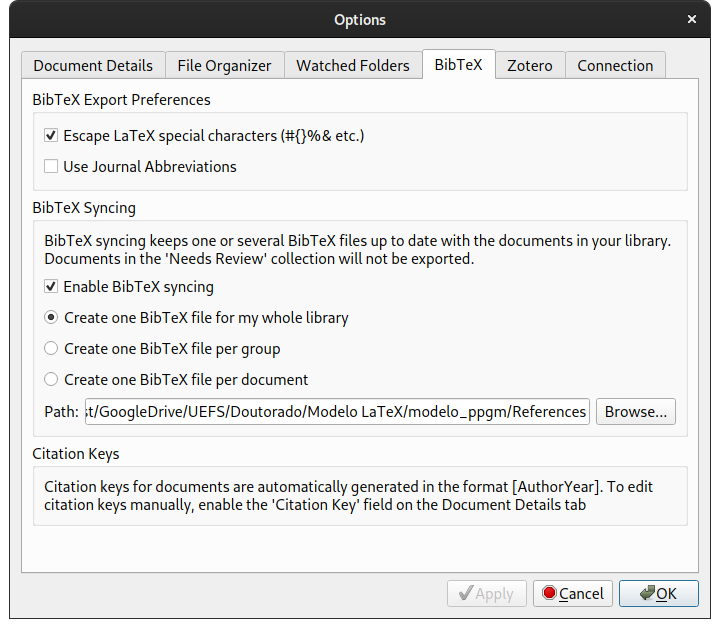
\includegraphics[scale=0.5]{Figures/bibtex_mendeley_desktop.png}
    \caption{Opções de exportação no Mendeley com suporte a BibTeX.}
    \label{fig:bibtex_mendeley_desktop}
\end{figure}

A base de dados Scopus também fornece uma opção para fazer o download das referências em BibTeX dos artigos selecionados na busca. Ele irá condensar todos os documentos em um único arquivo \verb=.bib=.

Outras ferramentas, como o JabRef, também farão o mesmo. Use-as para gerenciar os documentos e elas irão gerar um único arquivo \verb=.bib= com todos eles. No JabRef, você pode abrir os arquivos BibTeX que você baixou e depois condensá-los em um único arquivo. Esse arquivo único com todos os documentos será necessário no \LaTeX.

\subsection{Citando com o BibTeX}
\label{subsec:citando_com_bibtex}

Antes de mais nada, salve seu arquivo BibTeX com o nome \verb=referencias.bib= dentro da pasta \verb=References= deste projeto \LaTeX. Os comandos já especificados no arquivo principal deste projeto farão o carregamento das referências.

Com o arquivo BibTeX em seu devido lugar, basta usar os comandos \verb=\cite{}= e \verb=\citeonline{}= para fazer as citações, especificando a chave do documento. Os dois comandos variam na forma de apresentar a citação, conforme os dois exemplos abaixo.

Usando \verb=\cite{}=:

\begin{verbatim}
    Existe uma sub-notificação dos casos de COVID-19 no
    Brasil \cite{Costa2020}.
\end{verbatim}

Existe uma sub-notificação dos casos de COVID-19 no Brasil \cite{Costa2020}.

Usando \verb=\citeonline{}=:

\begin{verbatim}
    Segundo \citeonline{Costa2020}, existe uma sub-notificação dos casos
    de COVID-19 no Brasil.
\end{verbatim}

Segundo \citeonline{Costa2020}, existe uma sub-notificação dos casos de COVID-19 no Brasil.

Se a chave usada na citação não existir no arquivo de referências, será exibida uma interrogação no lugar. Preste atenção às chaves!

A lista de referências será gerada automaticamente ao final do documento seguindo a ordem alfabética (no caso da ABNT, em outros modelos, vai seguir a ordem definida pela revista ou instituição que criou o modelo). Tente citar outros documentos no arquivo \verb=referencias.bib= e verá que a lista é gerada corretamente.

\section{E agora?}
\label{sec:e_agora}

E agora você pode começar a escrever sua tese.

O documento original do modelo do PPGM sugere indicar como a tese/dissertação está estruturada, conforme exemplo abaixo:

``Tendo em vista o objetivo deste projeto, a dissertação foi organizada da seguinte forma, a contar da Introdução:

\begin{description}
    \item[Capítulo~\ref{cap:introducao} - Introdução] Introdução da pesquisa, seus objetivos, hipóteses, premissas...
    
    \item[Capítulo~\ref{cap:fund_teorica} - Fundamentação Teórica] Apresenta um estudo bibliográfico através de dados secundários...
    
    \item[Capítulo~\ref{cap:metodologia} - Metodologias] Apresenta a metodologia utilizada...
    
    \item[Capítulo~\ref{cap:conclusao} - Resultados e Conclusões] Apresenta os resultados obtidos na pesquisa e as conclusões...''
\end{description}

Procure seu orientador(a)! Os trabalhos devem seguir a ABNT NBR 14724:2011 (trabalhos acadêmicos). Algumas outras normas auxiliares podem ajudar:

\begin{itemize}
    \item NBR 6023:2018 - Referências bibliográficas
    \item NBR 6024:2012 - Numeração progressiva das seções de um documento
    \item NBR 6027:2012 - Sumário
    \item NBR 6028:2021 - Resumo
    \item NBR 10520:2002 - Citações
    \item NBR 12225:2004 - Lombada
\end{itemize}

Caso queira, pode pesquisar outras normas usando o catálogo da ABNT em \url{https://www.abntcatalogo.com.br/}.

Bom trabalho!

    \chapter{Fundamentação Teórica}
\label{cap:fund_teorica}

%%----------------------------------------------------------------------------
%% Escreva aqui o texto do seu capítulo. Verifique o título no comando
%% \chapter e lembre-se de dar um \label para ele. Adicione mais arquivos como
%% este caso precise de mais capítulos.
%%----------------------------------------------------------------------------

% O comando abaixo gera texto aleatório. Remova-o!
\lipsum[1-4]

    \chapter{Metodologia}
\label{cap:metodologia}

%%----------------------------------------------------------------------------
%% Escreva aqui o texto do seu capítulo. Verifique o título no comando
%% \chapter e lembre-se de dar um \label para ele. Adicione mais arquivos como
%% este caso precise de mais capítulos.
%%----------------------------------------------------------------------------

% O comando abaixo gera texto aleatório. Remova-o!
\lipsum[5-8]

    \chapter{Resultados e Conclusões}
\label{cap:conclusao}

%%----------------------------------------------------------------------------
%% Escreva aqui o texto do seu capítulo. Verifique o título no comando
%% \chapter e lembre-se de dar um \label para ele. Adicione mais arquivos como
%% este caso precise de mais capítulos.
%%----------------------------------------------------------------------------

% O comando abaixo gera texto aleatório. Remova-o!
\lipsum[9-12]

    % Caso precise de mais capítulos, basta criar novos arquivos e acrescentá-los
    % aqui seguindo o modelo acima

    %%----------------------------------------------------------------------------
    %% Inclui anexos
    %%----------------------------------------------------------------------------
    % Comente qualquer linha que não queira inserir
    \begin{thesisappendices}
        \chapter{Anexo I}
\label{anex1}
\begin{center}
    \textbf{Aqui pode ser um Título do seu Anexo}
\end{center}

Texto do Anexo.

        % Caso precise de mais anexos, basta criar novos arquivos e acrescentá-los
        % aqui seguindo o modelo acima
    \end{thesisappendices}

    %%----------------------------------------------------------------------------
    %% Configurar as referencias bibliográficas
    %%----------------------------------------------------------------------------
    \addcontentsline{toc}{chapter}{Referências}
    %\bibliographystyle{abntex2}
    %\bibliographystyle{unsrt}
    %\bibliographystyle{abnt}
    \bibliography{References/referencias}
    
    %%----------------------------------------------------------------------------
    %% Finalização
    %%----------------------------------------------------------------------------
    %==========================================================
%        Document: PPGM-UEFS
%        File....: UltimaFolha.TEX
%        Author..: Gilney Zebende
%        Date....: 24 de abril de 2018
%==========================================================
\begin{ultimafolha}

\vspace*{\fill}

\begin{flushleft}
{\it \thetitle} \\
\ \\
\theauthor \\
\ \\
\ppgmcidade, \ppgmmes\space de \ppgmano.
\end{flushleft}
\end{ultimafolha}

\end{document}

%%%-------------------------------------------------------------------------------
%%% Aqui finalizamos a formatação. Faça um bom trabalho.
%%%-------------------------------------------------------------------------------
